\documentclass{article}
\usepackage[utf8]{inputenc}
\usepackage{multicol}
\setlength\columnsep{20pt}
\usepackage{listings}
\usepackage{geometry}
\usepackage{color}
\usepackage{float}
\setlength{\belowcaptionskip}{-10pt}
\setlength{\abovecaptionskip}{-30pt}
\floatstyle{boxed} 
\restylefloat{figure}
\usepackage{hyperref}
\usepackage{graphicx}
\definecolor{codegreen}{rgb}{0,0.6,0}
\definecolor{codegray}{rgb}{0.5,0.5,0.5}
\definecolor{codepurple}{rgb}{0.58,0,0.82}
\definecolor{backcolour}{rgb}{0.95,0.95,0.92}

\lstdefinestyle{mystyle}{
	backgroundcolor=\color{backcolour},   
	commentstyle=\color{codegreen},
	keywordstyle=\color{blue},
	numberstyle=\tiny\color{codegray},
	stringstyle=\color{codepurple},
	basicstyle=\footnotesize,
	breakatwhitespace=false,         
	breaklines=true,                 
	captionpos=b,                    
	keepspaces=true,                 
	numbers=left,                    
	numbersep=5pt,                  
	showspaces=false,                
	showstringspaces=false,
	showtabs=false,                  
	tabsize=2
}

\lstset{style=mystyle}
\title{Data Mining\\ Home Work 03}
\author{aqeel labash}
\date{24 February 2016}
\geometry{
	a4paper,
	total={170mm,257mm},
	left=5mm,
	top=5mm,
	right=5mm
}
\begin{document}
	\maketitle
		{\centering \section*{First Question}}
\begin{flushleft}
To plot the density I used the following code : 
\begin{lstlisting}[language=R]
##### Question 1 #####
rm(list=ls())
setwd("/home/aqeel/Study/DM/HW03")
klient1 <- read.csv('klien	t1.txt',header = FALSE)
klient3 <- read.csv('klient3.txt',header=FALSE)
png("densitywithoutwidth.png",width=500,height = 500)
plot(density(klient1$V1),col="RED",type = "l",main="K1 & K3 Density")
lines(density(klient3$V1),col="green")
dev.off()
\end{lstlisting}

The previous code will plot the density of klient1 \& klient3 without specifying the bandwidth. We notice that there is only a small difference between klient1 and klient3.
\begin{figure}[H]
\begin{center}
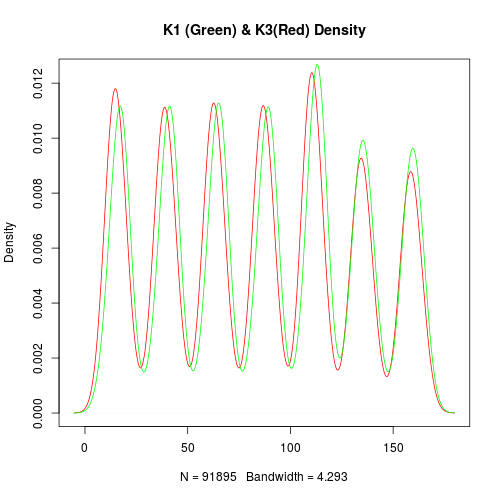
\includegraphics[scale=0.7]{densitywithoutwidth.png}
\end{center}
\caption{Show the density of K1 \& K3 without specifying width}
\end{figure}
Now to choose the width actually I tried the values to reach a level where I can see the gaps without this periodic behavior in the density. I selected bandwidth to be 11 where we still can see the changes but it won't affect our judgment of the data (high points,small points etc..).Here is the figure with bandwidth:
\begin{figure}[H]
	
\begin{center}
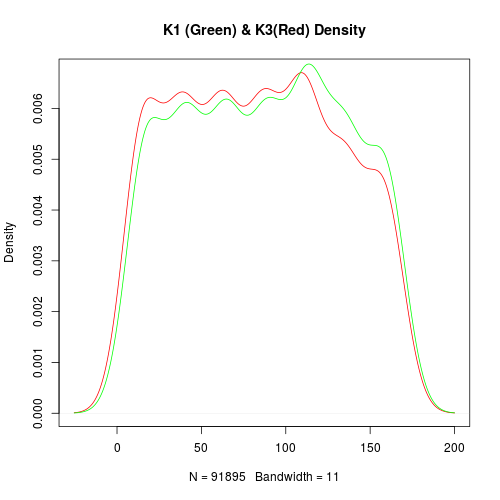
\includegraphics[scale=1]{densitywithwidth.png}
\end{center}
\caption{Shows K1\&K3 density with specified bandwidth}
\end{figure}
Figure 2 was generated by the following code : 
\begin{lstlisting}[language=R]
png("densitywithwidth.png",width = 500,height = 500)
bandwidth =11
plot(density(klient1$V1,bw=bandwidth,kernel = "gaussian"),col="RED",type = "l",main="K1 (Green) & K3(Red) Density")
lines(density(klient3$V1,bw=bandwidth,kernel = "gaussian"),col="green")
dev.off()
\end{lstlisting}
\end{flushleft}
To characterize the data first we should understand the data.
Week hours  : 7*24= 168 , that's how the time is identified. And the holiday is from 120 to 168.So depending on that information here is some characteristics about the data:
\begin{enumerate}
	\item Both groups shows higher activity at the start of week end.
	\item Both groups shows less activity at the week start.
	\item First group (in Green) shows less active during the week than second group (K3,in red)
	\item First group shows more activity at the start of weekend than the second group.
	\item There is a slight shift between both groups.Which made me think that the groups from different time zones
\end{enumerate}
		{\centering \section*{Second Question}}					\begin{flushleft}
		The data contain the following information : 
		\begin{enumerate}
			\item Date:the date of purchase in syntax of : "YYYYMMDD"
			\item Time:the time of purchase in syntax of : "HHMM" or "HMM" depending on time.The time is based on 24 not 12.
			\item Product: the name of the product.
			\item Shope\_id: represent the shop identity
		\end{enumerate}	
		The following Table shows : 
		\begin{enumerate}
			\item How many products bought from specific shop.
			\item The total amount bought of specific product from all the shops.
			\item The total amount bought from specific shop.
			\item The total bought from all shops from all products.
		\end{enumerate}
		\begin{tabular}{|c|c|c|c|c|c|c|}
			\hline
Product\textbackslash Shop&3&4&18&21&32& Total\\ \hline
Banana&6778&8677&4080&1727&3585&24847\\ \hline
Coffee\_Cream&4272&7259&4516&1418&3066&20531\\ \hline
Eggs\_1&1880&3704&1326&1106&2073&10089\\ \hline
Eggs\_2&100&181&0&0&0&281\\ \hline
Grapes&710&1199&495&273&525&3202\\ \hline
Milk\_1&3568&5173&2740&836&2557&14874\\ \hline
Milk\_2&5629&8309&4968&2440&4369&25715\\ \hline
Sour\_Cream\_1&2597&3206&1817&848&1236&9704\\ \hline
Sour\_Cream\_2&2891&5504&3046&1569&2866&15876\\ \hline
Vastlakukkel&939&1784&730&273&383&4109\\ \hline
Whipped\_Cream&2285&3815&1168&600&1396&9264\\ \hline
Total&31649&48811&24886&11090&22056&138492\\ \hline
		\end{tabular}
		
		The code used to generate the previous table is here:
		\begin{lstlisting}[language=R]
		shopsdata = read.csv("product_time_shop.txt",sep = ';',header = TRUE)
		x<-table(shopsdata$product,shopsdata$shop_id)
		x<-cbind(x,rowSums(x))
		x<-rbind(x,colSums(x))
		x
		\end{lstlisting}
	\end{flushleft}

		{\centering \section*{Third Question}}
To create the boxplots I depended on the 2nd question result.
in Figure 1 we can notice that Tuesday has the highest selling over all products. I guess that's because people misjudged there needs at the start of the week :) (am not alone :D ).Saturday also has a high sell rate over all products. Which could be explained by holiday \& people buying for the week.
\begin{figure}[H]
	\begin{center}
		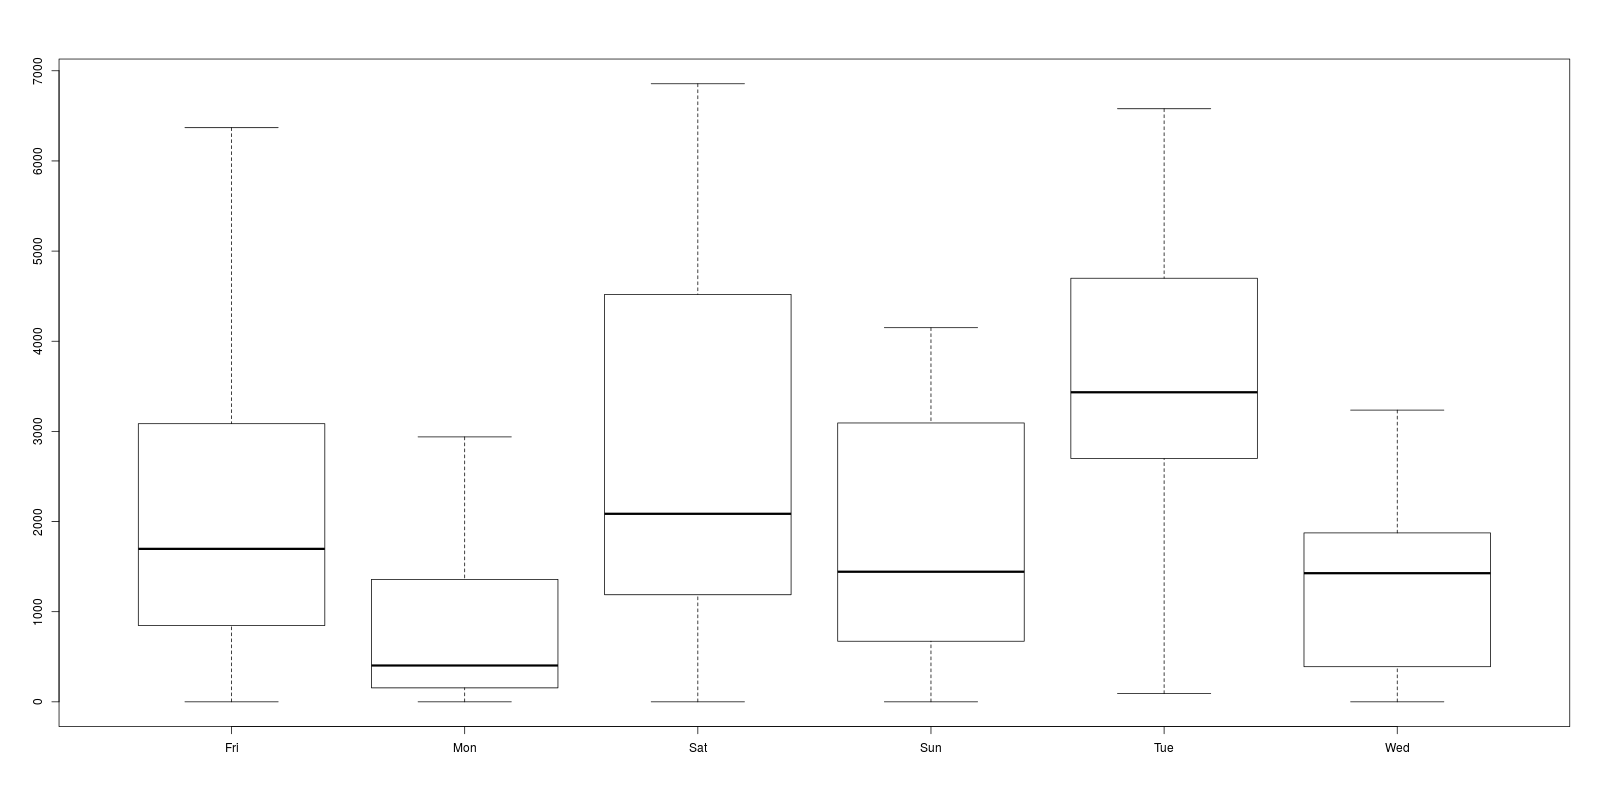
\includegraphics[scale=0.3]{boxplotdates.png}
	\end{center}
	\caption{Total sales in the specified dates in all stores (Date~Product)}
\end{figure}
In figure 2 we can see that Milk\_2 has a high median which mean it's most sold in most stores.
the opposite for Eggs\_2 \& Grapes which mean they haven't sold much.Banana have a high selling over most of the stores.
\begin{figure}[H]
\begin{center}
	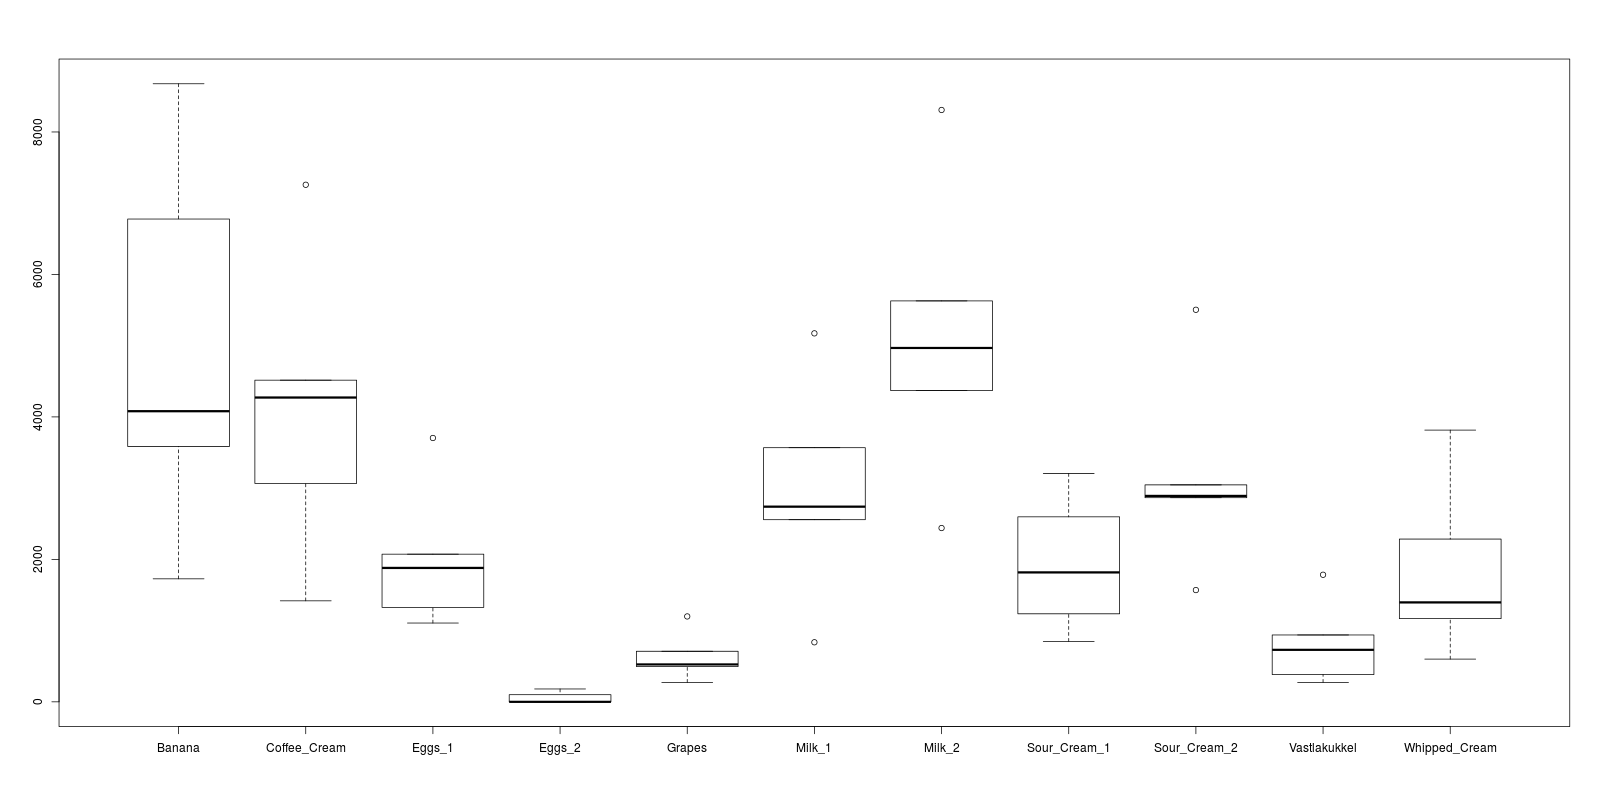
\includegraphics[scale=0.3]{boxplotproducts.png}
\end{center}
\caption{Total sold products in all dates , all stores.(Product ~ Store)}
\end{figure}
Figure 3 shows us the most product where bought from "Store 4". Also "Store 21" didn't sell much of the products compared to other stores.
\begin{figure}[H]
\begin{center}
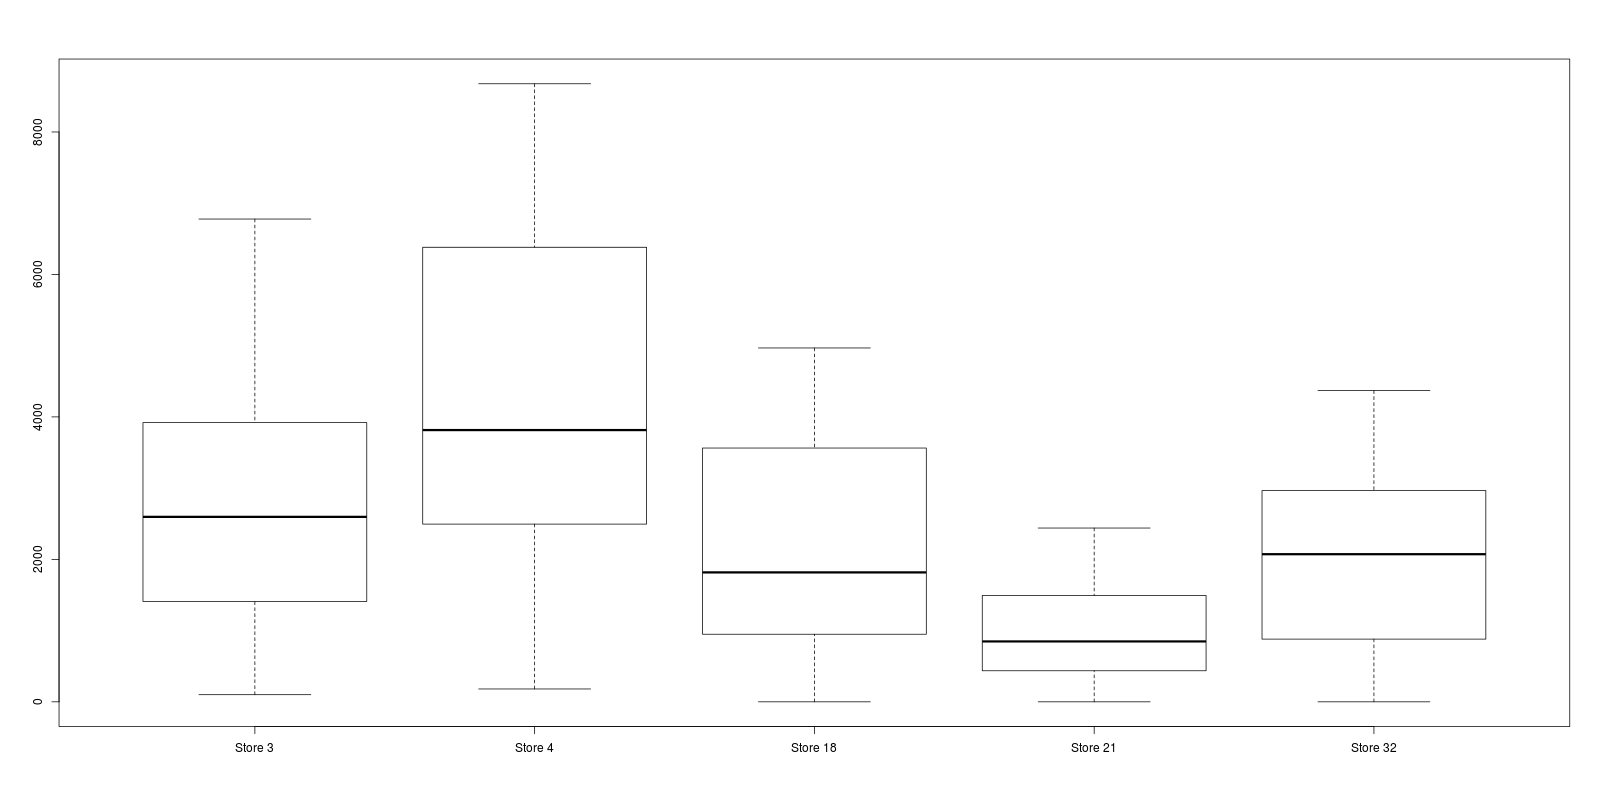
\includegraphics[scale=0.3]{boxplotStores.png}
\end{center}
\caption{Total sales in specific store in all dates , all products (Store ~ Product)}
\end{figure}

The previous boxplots where generated by this code :
\begin{lstlisting}[language=R]
##### Third Question ##########
library(plyr)
days<-c("Sat","Sun","Sat","Tue","Mon","Tue","Sun","Sat","Fri","Fri","Tue","Wed")
shopsdata$date<- mapvalues(shopsdata$date, from = c(unique(shopsdata$date)), to = days)
png("boxplotStores",width=1600,height = 800)
boxplot(x[,(1:5)],names=paste("Store",colnames(x),sep=" "))
dev.off()
png("boxplotproducts",width = 1600,height = 800)
boxplot(t(x)[,(1:11)],names=colnames(t(x)))
dev.off()
png("boxplotdates.png",width=1600,height=800)
boxplot(table(shopsdata$product,shopsdata$date)[,c(1:6)])
dev.off()
\end{lstlisting}
To represent the data I created a plot compare store vs product.:
\begin{figure}[H]
\begin{center}
	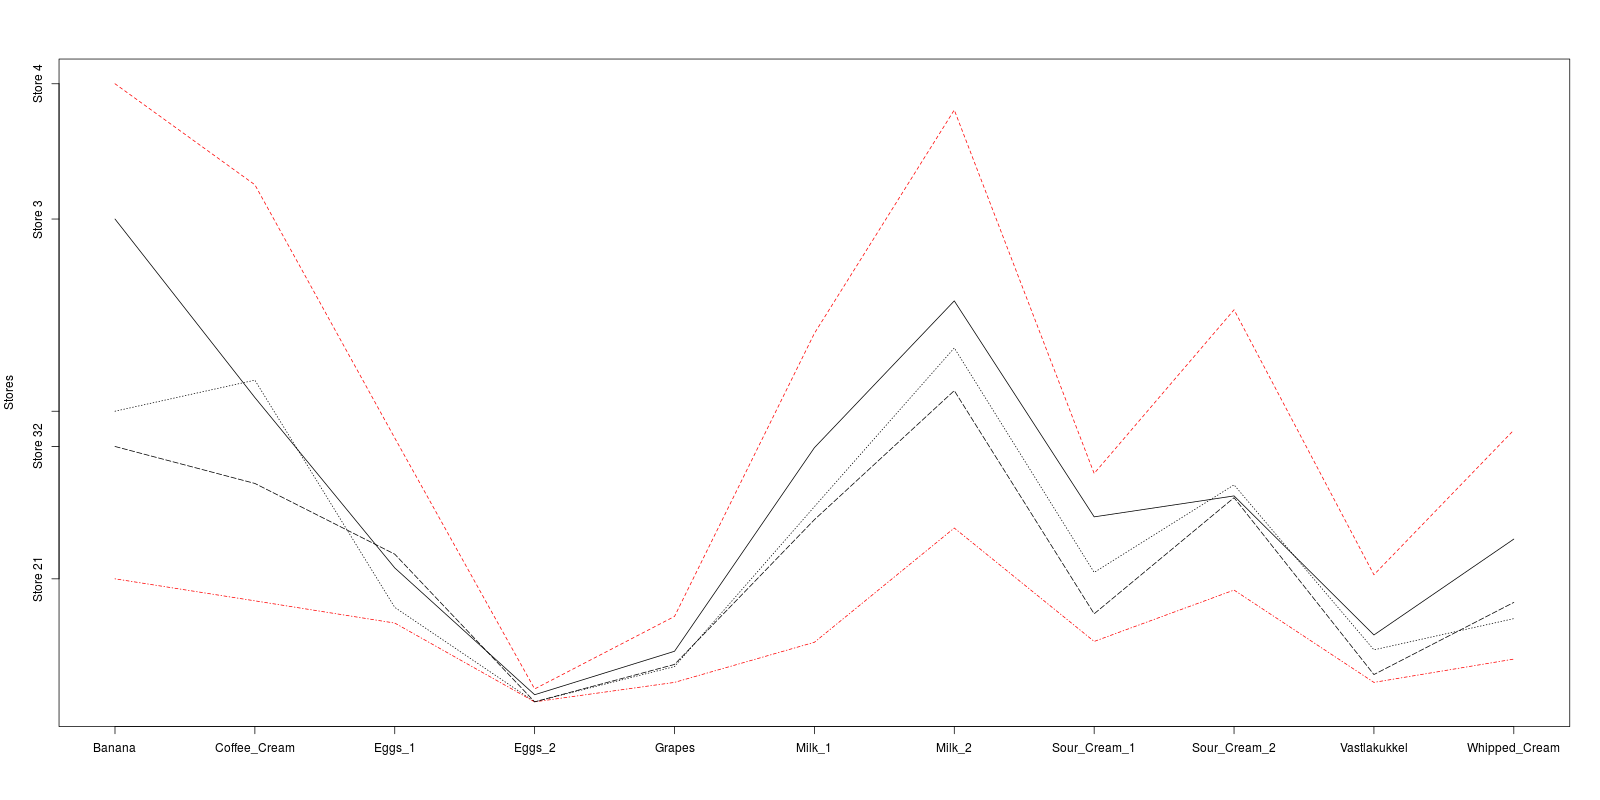
\includegraphics[scale=0.3]{matplotallvsall.png}
\end{center}
\caption{Stores vs products}
	
\end{figure} 
From the previous figure we can see that store 4 was selling the most.Banana and milk\_2 was the most sold thing. I believe this figure satisfy information wanted from stores and products.
The previous plot was generated by the following code : 
\begin{lstlisting}[language=R]
png("matplotallvsall.png",width=1600,height=800)
matplot(x, pch = 16,  col = 1:2,xaxt="n",yaxt="n",
ylab = "Stores",type = "l")
axis(1,at=c(1:11),labels = rownames(x))
axis(2,at=x[1,],labels =paste("Store",colnames(x),sep=" "))
dev.off()
\end{lstlisting}
		{\centering \section*{Fourth Question}}
For this task  I looked at the data. We can know if a specific store run out of some or one product if this products stopped selling while the rest still.So I wrote some code to see this fact and here is the code :
\begin{lstlisting}[language=R]
######## Fourth Question #################
shopsdata = read.csv("product_time_shop.txt",sep = ';',header = TRUE)
products <- unique(shopsdata$product)

dd <-subset(shopsdata,date=="20140104" & shop_id==18)[,(2:3)]
dd$product<- factor(dd$product,products,c(1:11))
png("distribution.png",width = 900,height = 1100)
plot(dd,yaxt="n",main="Store 18 at  2014/01/04")
axis(2,at=c(1:11),labels =products)
dev.off()
dd<-subset(dd,product==9)
png("histdensity.png",width = 600,height = 600)
hist(dd$time,prob=TRUE,xlim =c(1000,2400),main = "Density Over Histogram",xlab="Time")
lines(density(dd$time),col="RED")
dd <-subset(shopsdata,date=="20140104" & shop_id==18)[,(2:3)]
dd$product<- factor(dd$product,products,c(1:11))
dd<-subset(dd,product==8)

lines(density(dd$time),col="GREEN")
dev.off()

\end{lstlisting}
The previous code will plot figure 5 which show the distribution of products over time in Store 18 at 2014/01/04. That allow us to see when a product is not sold anymore while other products still being sold.
Same figure show us that product Milk\_2 stopped selling around 16~18 (not accurate due lake of space in the image.) 
\begin{figure}[H]
\begin{center}
	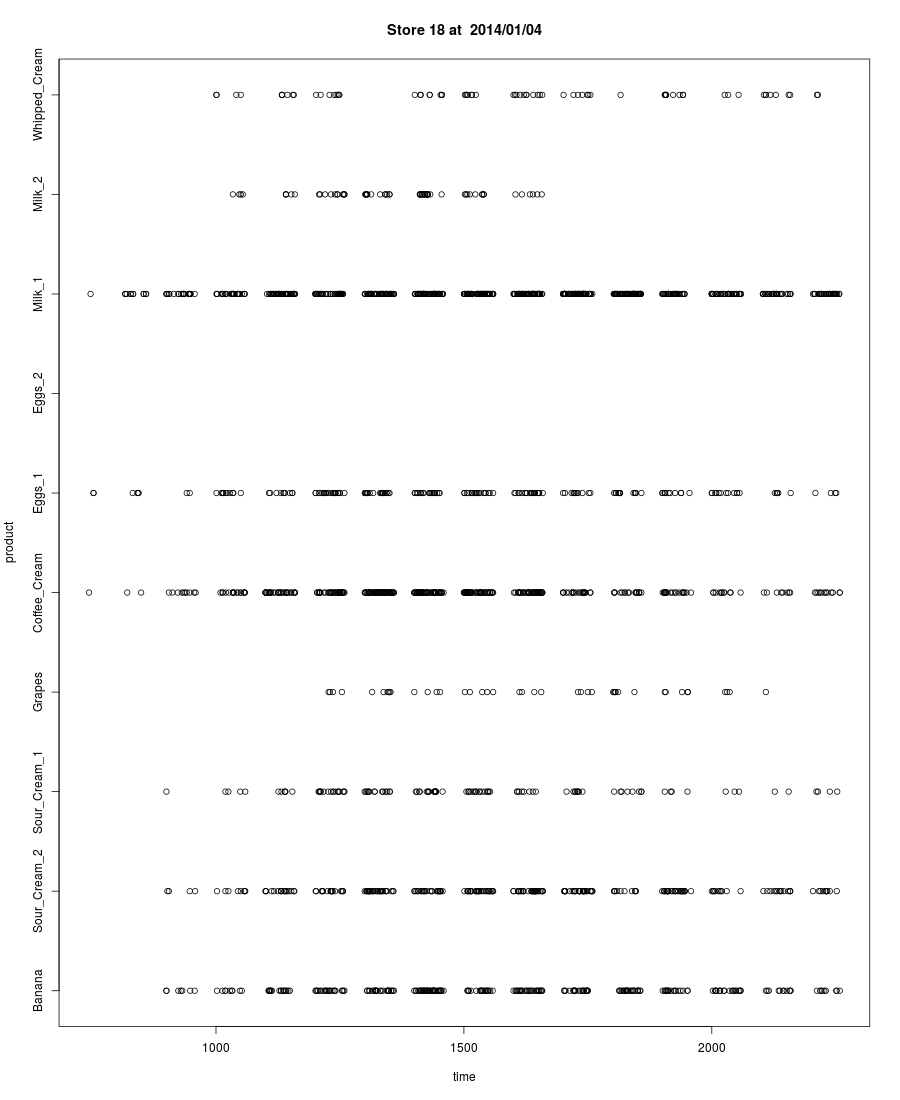
\includegraphics[scale=0.6]{distribution.png}
\end{center}
\caption{Show the time of selling all products.}
\end{figure}
\begin{flushleft}

After that to convince you more here is a figure 6 which contain the histogram and the density over it. The red line is Milk\_2 and the green line is Milk\_1 and we can clearly see that after 1700 o'clock there was no more purchases over milk\_2.
\begin{figure}[H]
\begin{center}
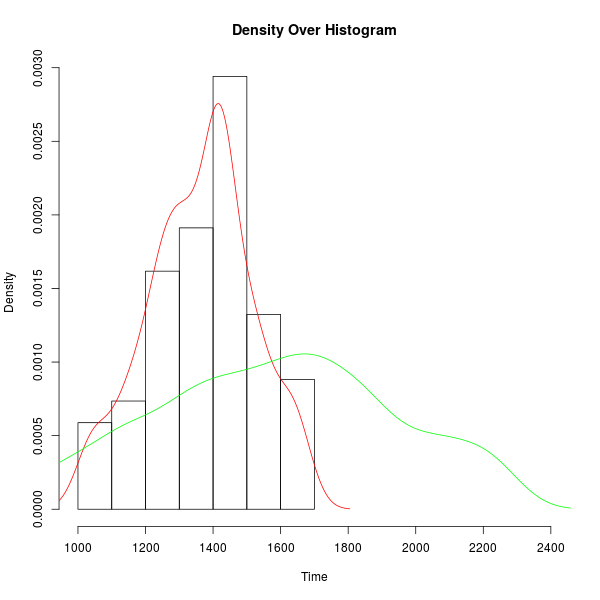
\includegraphics[scale=0.8]{histdensity.png}
\end{center}
\caption{Milk\_2 density (in red) vs Milk\_1 density (green)}
\end{figure}
So to formulate it, we can check by fix date,store and then check over all products in one hit to see which one doesn't sell at specific time while other products still selling.
\end{flushleft}
		{\centering \section*{Fifth Question}}
For this question what I've done is firstly organize the data.So I concatenated the columns (Date,Product,Store) after that I updated the time value then draw the heat map.
and here is the code : 
\begin{lstlisting}[language=R]
############ Question 5 ##############
rm(list=ls())
shopsdata = read.csv("product_time_shop.txt",sep = ';',header = TRUE)
shopsdata$info=paste(paste(shopsdata$date, shopsdata$product, sep=";"),shopsdata$shop_id,sep = ";")
shopsdata$date=NULL
shopsdata$product=NULL
shopsdata$shop_id=NULL
for (i in c(7:23))
{
shopsdata[shopsdata$time>=(i*100)&shopsdata$time<((i+1)*100),]$time =i
}
colSums(table(shopsdata$info,shopsdata$time))
png("heatmap2.png",width=800,height = 800)
heatmap(table(shopsdata$info,shopsdata$time))
dev.off()
\end{lstlisting}
Here is the heatmap :
\begin{figure}[H]
\begin{center}
	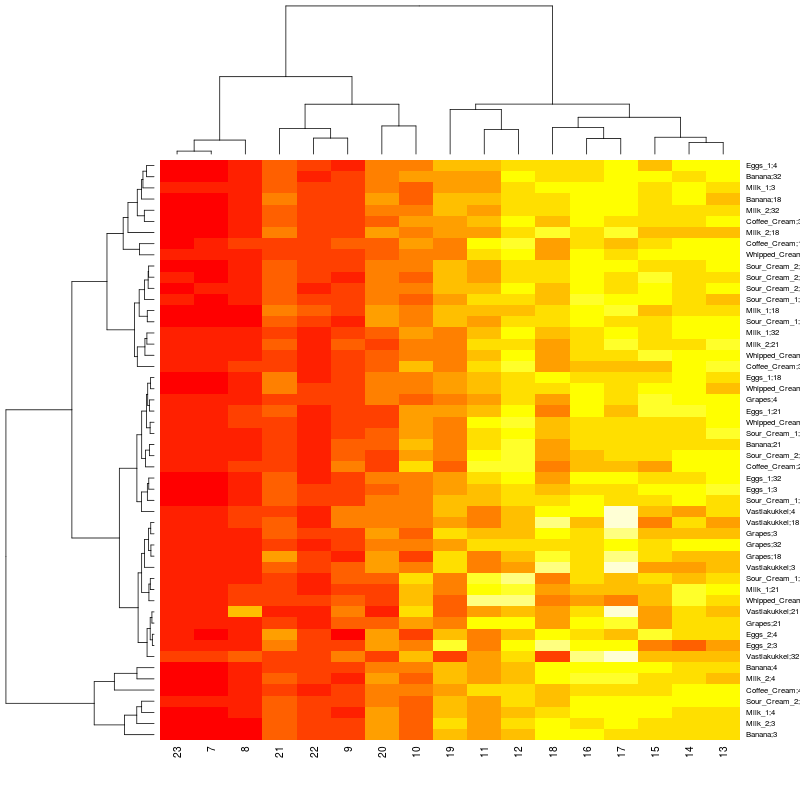
\includegraphics[scale=0.7]{heatmap2.png}
\end{center}
\caption{Heatmap (Red to Yellow)}
\end{figure}
\begin{flushleft}

In figure 7 the heat map shows that at 13 (1 PM) it's the most time that people buy in general.\\
\textbf{Note:} In the heat map the time ordered depending on heat.At 23 the less heat but at 13 the highest heat.
\end{flushleft}
		{\centering \section*{Sixth Question}}
		{\centering \subsection*{(1)}}
		\begin{flushleft}

To see the behavior, I firstly replaced the dates with week days and then calculated the total sales per day using the following code :
\begin{lstlisting}[language=R]
\end{lstlisting}
The previous code create the following table : \\
\begin{tabular}{|c|c|c|c|c|c|c|}
	\hline
Fri&Mon&Sat&Sun&Tue&Wed\\
\hline
23948&9649&32260&20460&38174&14001\\
\hline
\end{tabular}\\
where we can see that people usually by more on Saturday and that's clear and expected. The shock come from Tuesday which has a high selling rate.I think this high value is due to end of what usually people buy on the week end.Here is the code I used for this task:
\begin{lstlisting}[language=R]
############### Question 6 ##############
###1st request###
rm(list=ls())
setwd("/home/aqeel/Study/DM/HW03")
shopsdata = read.csv("product_time_shop.txt",sep = ';',header = TRUE)
library(plyr)
days<-c("Sat","Sun","Sat","Tue","Mon","Tue","Sun","Sat","Fri","Fri","Tue","Wed")
shopsdata$date<- mapvalues(shopsdata$date, from = c(unique(shopsdata$date)), to = days)
\end{lstlisting}
\end{flushleft}
		{\centering \subsection*{(2)}}
To do that I used the table of Days-Products.To normalize we can take the maximum value in the matrix and divide the matrix over that number.Here is the code for this request:
\begin{lstlisting}[language=R]
###2nd request###
products_shops<-table(shopsdata$date,shopsdata$product)
products_shops<- products_shops/norm(products_shops,type ="M")
png("heatmapproductsvsdays.png",width = 500, height = 500)
heatmap(products_shops)
dev.off()
\end{lstlisting}
After that I created a heat map to have a clear view of products bought which day.
\begin{figure}[H]
	\begin{center}
		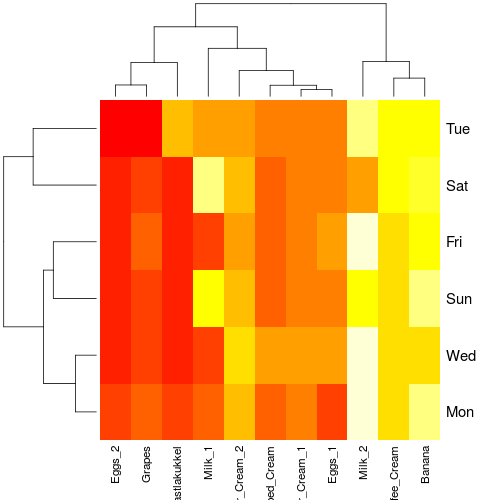
\includegraphics[scale=1]{heatmapproductsvsdays.png}
	\end{center}
	\caption{Shows heat map of products over week days}
\end{figure}
		{\centering \subsection*{(3)}
\begin{flushleft}
For this task I changed the data:(dates to week days , time to formual hour, merged date with time ) after that created a table (too large 100 row ). Then I normalized the matrix and table it to get the following plot:
\begin{figure}[H]
	\begin{center}
		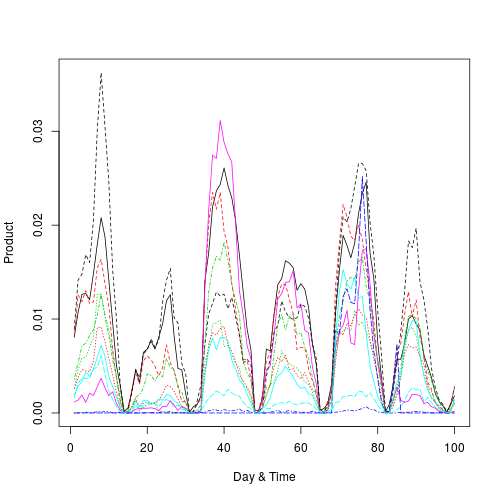
\includegraphics[scale=0.9]{frequencyoverdays.png}
	\end{center}
	\caption{Product vs day and time.}
\end{figure}
Here is the code for this task : 
\begin{lstlisting}[language=R]
###3rd request###
for (i in c(7:23))
{
shopsdata[shopsdata$time>=(i*100)&shopsdata$time<((i+1)*100),]$time =i
}
days<-c("Sat","Sun","Sat","Tue","Mon","Tue","Sun","Sat","Fri","Fri","Tue","Wed")
shopsdata$date<- mapvalues(shopsdata$date, from = c(unique(shopsdata$date)), to = days)
shopsdata$date<-paste(shopsdata$date, shopsdata$time, sep=" ")
shopsdata$time<-NULL
products_overtime <-table(shopsdata$date,shopsdata$product)
products_overtime<- products_overtime/norm(products_overtime)
png("frequencyoverdays.png",width=500,height=500)
matplot(products_overtime,type = "l",xlab = "Day & Time" , ylab = "Product" )
dev.off()
\end{lstlisting}
{\centering\subsection*{(4)}}
From the previous figure which shows the products bought at specific day\& time.\\
I believe if we have it large enough to identify the axis we would be able to identify the products that sold out.
\end{flushleft}
\end{document}